\chapter{Coordinate System}
\section{Rectangular Coordinate System}
\textbf{Coordinates of a point} is how each point on a plane is assigned a pair of numbers.\\
\textbf{Origin} is the point of \textit{intersection} of the x-axis and y-axis.\\
\textbf{Coordinate Plane} is the x-axis, y-axis, and all the points in their plane.\\
\textbf{Ordered Pairs} is a pair of numbers, written in parethesis and separated by comma for a point. Every point on a coordinate plane determined by order of numbers. example being (0,0) for the origin.\\
\textbf{X-Coordinate} is the number to the left of the comma in an ordered pair and determines the movement along the x-axis from origin. It moves right for positive and left for negative.\\
\textbf{Y-Coordinate} is the number to the right of the comma in an ordered pair and determines the movement perpendicular from the x-coordinate. It moves above the x-coordinate for positive and below the x-coordinate for negative.
\\
\textbf{Quadrants} are the four separated regions of a coordinate plane. Starting on top right and going counter-clockwise they're are named Quadrant I-IV.\\
\textbf{Graph} is the point associated with an ordered pair of real numbers.

\subsection{Distance Formula}
\begin{center}
	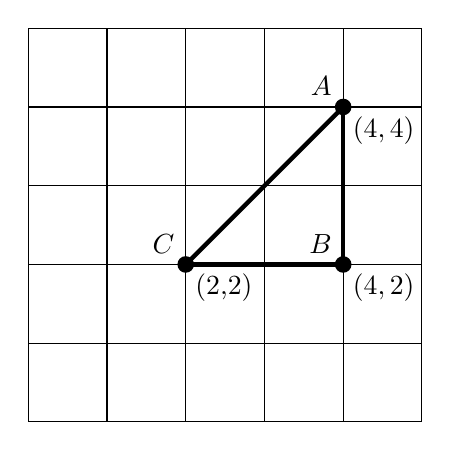
\begin{tikzpicture}
		\draw (0,0) grid (5,5);
		\draw[ultra thick] (2,2) -- (4,2) node[above left] {$B$};\fill (2,2) circle (3pt) node[below right] { (2,2) };
		\draw[ultra thick] (4,2) -- (4,4) node[above left] {$A$};\fill (4,2) circle (3pt) node[below right] {$(4,2)$};
		\draw[ultra thick] (4,4) -- (2,2) node[above left] {$C$};\fill (4,4) circle (3pt) node[below right] {$(4,4)$};
	\end{tikzpicture}

\end{center}

\begin{equation}
	d = \sqrt{(x_2 - x_1)^2 + (y_2 - y_1)^2}	
\end{equation}

All distances can be found by subtracting, except the \textit{hypotenuse}, which is found using the \textbf{Pythagorean Formula}.

\subsection{Midpoint Formula}
\begin{center}
	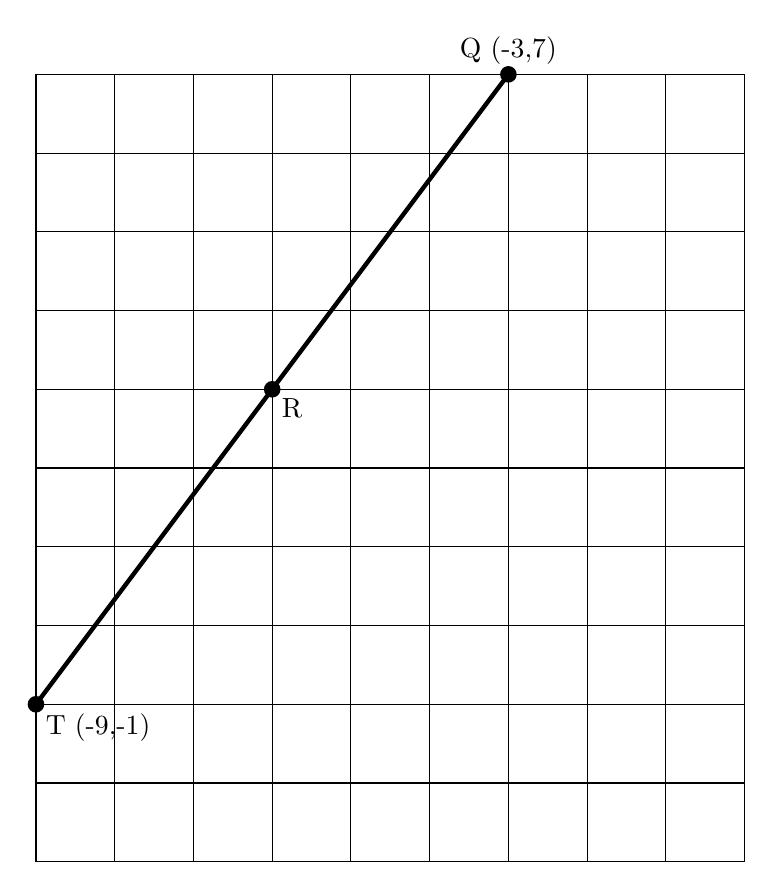
\begin{tikzpicture}
		\draw (-9,-3) grid (0,7);
		\draw[ultra thick] (-9,-1) -- (-3,7); \fill (-9,-1) circle (3pt) node[below right] {T (-9,-1) };
		\fill (-3,7) circle (3pt) node[above] {Q (-3,7)};
		\fill (-6,3) circle (3pt) node[below right] {R};
	\end{tikzpicture}
\end{center}

\begin{equation}
	M = (\frac{x_1 + x_2}{2},\frac{y_1 + y_2}{2})
\end{equation}

\textbf{Midpoint} is the average of the endpoints.

\newpage
\subsection{Slope of a Line}

\begin{center}
	\begin{tikzpicture}
		\begin{axis}[standard, 
			xtick={-7,-6,-5,-4,-3,-2,-1,0,1,2,3,4,5,6},
			ytick={-4,-3,-2,-1,0,1,2,3,4,5},
			samples=1000,
			xlabel={$x$},
			ylabel={$y$},
			xmin=-7,xmax=6,
			ymin=-4,ymax=5,
			clip=false]

			% horizontal line - a
			\addplot[
				<->,
				blue,  
				thick, 
				domain=-7:6,
				samples=2
				] {3} node[anchor=south] {$a$};

			\addplot[
				<->,
				gray,  
				thick
				] coordinates {(-2, -4) (-2, 5)} node[anchor=south] {b};

			\addplot[
				<->,
				thick,
				] {x+2} node[anchor=south] {c};

		\end{axis}
	\end{tikzpicture}
\end{center}
\[
	\boxed{m = \dfrac{y_2 - y_1}{x_2 - x_1}}
\]

The \textbf{slope of a line} is a measurement of steepness and direction of a \textit{nonvertical} line. This means line \textbf{b} has an undefined slope, while slope \textbf{a} has a slope of 0.
Meanwhile, \textbf{c} has an x-intercept at -2 and a y-intercept at 2. These intercepts are when either x or y are equal to 0.

\newpage
\subsection{Slopes of Parallel and Perpendicular Lines}
\textbf{Parallel} lines have equal slopes and \textbf{Perpendicular} lines have \textit{opposite} slopes/their product is -1. \\

\textbf{Example:} 
Given the original slope:
$$m = \frac{3}{4}$$

The slope of a parallel line ($m_{\parallel}$) is the same:
$$m_{\parallel} = \frac{3}{4}$$

The slope of a perpendicular line ($m_{\perp}$) is the negative reciprocal:
$$m_{\perp} = -\frac{4}{3}$$

\subsection{Equations of Lines}
\textbf{1.} If a point lies on the graph of an equation, then its coordinates make the equation true, and \\\\
\textbf{2.} If the coordinates of a point make an equation a true statement, then the point lies on the graph of the equation.

They can be written in the form of Ax + By = C, where A \& B are not zero. If they were zero then C would always have to be zero too making the form false.

\textbf{Standard Form} is $Ax + By = C$ for the equation of a line. \\
\textbf{X-Intercept} is where the y-coordinate is 0. \\
\textbf{Y-Intercept} is where the x-coordinate is 0. \\

\textbf{Note:} Horizontal lines have no x-intercept unless its on the x-axis.\\Vertical lines have no y-intercept unless its on the y-axis.

\subsection{Graphs of Linear Inequalities}
\textbf{Linear Inquality} is a sentence in the form of $Ax + By < C$. This can be any less than, greater than, or less/greater than or equal to symbol.
\\\\
If it is 'or equal to' then you make the line solid when graphing.\\ If it is not, then you make the line dotted as a boundary. This is because you are not counting what is on the line. 
\\\\
Now you want to plot a test point that is \textit{not} on the line. If this test point is true for the inequality then shade the side it is on, if not, shade the opposite side if it is false.
